%% ----------------------------------------------------------------
%% Thesis.tex -- MAIN FILE (the one that you compile with LaTeX)
%% ---------------------------------------------------------------- 

% Set up the document
\documentclass[a4paper, 11pt, oneside]{Thesis}  % Use the "Thesis" style, based on the ECS Thesis style by Steve Gunn
\graphicspath{Figures/}  % Location of the graphics files (set up for graphics to be in PDF format)

% Include any extra LaTeX packages required
\usepackage[square, numbers, comma, sort&compress]{natbib}  % Use the "Natbib" style for the references in the Bibliography
\usepackage{verbatim}  % Needed for the "comment" environment to make LaTeX comments
\usepackage{vector}  % Allows "\bvec{}" and "\buvec{}" for "blackboard" style bold vectors in maths
\usepackage{minted}
\hypersetup{urlcolor=blue, colorlinks=false}  % Colours hyperlinks in blue, but this can be distracting if there are many links.

%% ----------------------------------------------------------------
\begin{document}
\frontmatter      % Begin Roman style (i, ii, iii, iv...) page numbering

% Set up the Title Page
\title  {Optimal Team Formation in Fantasy Basketball}
\authors  {{Anthony Mazzawi}}
\addresses  {\groupname\\\deptname\\\univname}  % Do not change this here, instead these must be set in the "Thesis.cls" file, please look through it instead
\date       {September 2017}
\subject    {}
\keywords   {}

\maketitle
%% ----------------------------------------------------------------

\setstretch{1.3}  % It is better to have smaller font and larger line spacing than the other way round

% Define the page headers using the FancyHdr package and set up for one-sided printing
\fancyhead{}  % Clears all page headers and footers
\rhead{\thepage}  % Sets the right side header to show the page number
\lhead{}  % Clears the left side page header

\pagestyle{fancy}  % Finally, use the "fancy" page style to implement the FancyHdr headers

%% ----------------------------------------------------------------
% Declaration Page required for the Thesis, your institution may give you a different text to place here
\Declaration{

\addtocontents{toc}{\vspace{1em}}  % Add a gap in the Contents, for aesthetics

I, Anthony Mazzawi, declare that this thesis titled, `Optimal Team Formation in Fantasy Basketball' and the work presented in it are my own. I confirm that:

\begin{itemize} 
\item[\tiny{$\blacksquare$}] This work was done wholly or mainly while in candidature for a research degree at this University.
 
\item[\tiny{$\blacksquare$}] Where any part of this thesis has previously been submitted for a degree or any other qualification at this University or any other institution, this has been clearly stated.
 
\item[\tiny{$\blacksquare$}] Where I have consulted the published work of others, this is always clearly attributed.
 
\item[\tiny{$\blacksquare$}] Where I have quoted from the work of others, the source is always given. With the exception of such quotations, this thesis is entirely my own work.
 
\item[\tiny{$\blacksquare$}] I have acknowledged all main sources of help.
 
\item[\tiny{$\blacksquare$}] Where the thesis is based on work done by myself jointly with others, I have made clear exactly what was done by others and what I have contributed myself.
\\
\end{itemize}
 
 
Signed:\\
\rule[1em]{25em}{0.5pt}  % This prints a line for the signature
 
Date:\\
\rule[1em]{25em}{0.5pt}  % This prints a line to write the date
}
\clearpage  % Declaration ended, now start a new page

%% ----------------------------------------------------------------
% The "Funny Quote Page"
%\pagestyle{empty}  % No headers or footers for the following pages

%\null\vfill
% Now comes the "Funny Quote", written in italics
%\textit{``Write a funny quote here.''}

%\begin{flushright}
%If the quote is taken from someone, their name goes here
%\end{flushright}

%\vfill\vfill\vfill\vfill\vfill\vfill\null
%\clearpage  % Funny Quote page ended, start a new page
%% ----------------------------------------------------------------

% The Abstract Page
\addtotoc{Abstract}  % Add the "Abstract" page entry to the Contents
\abstract{
\addtocontents{toc}{\vspace{1em}}  % Add a gap in the Contents, for aesthetics

This will be a dissertation on the optimal team formation in fantasy basketball.  The first step is to predict match scores using the dixon model. ntasy basketball.  The first step is to predict match scores using the dixon model. ntasy basketball.  The first step is to predict match scores using the dixon model. ntasy basketball.  The first step is to predict match scores using the dixon model.ntasy basketball.  The first step is to predict match scores using the dixon model.
ntasy basketball.  The first step is to predict match scores using the dixon model.
ntasy basketball.  The first step is to predict match scores using the dixon model.
ntasy basketball.  The first step is to predict match scores using the dixon model.
ntasy basketball.  The first step is to predict match scores using the dixon model.ntasy basketball.  The first step is to predict match scores using the dixon model.
ntasy basketball.  The first step is to predict match scores using the dixon model.
ntasy basketball.  The first step is to predict match scores using the dixon model.
ntasy basketball.  The first step is to predict match scores using the dixon model.ntasy basketball.  The first step is to predict match scores using the dixon model.ntasy basketball.  The first step is to predict match scores using the dixon model.ntasy basketball.  The first step is to predict match scores using the dixon model.vntasy basketball.  The first step is to predict match scores using the dixon model.
}

\clearpage  % Abstract ended, start a new page
%% ----------------------------------------------------------------

\setstretch{1.3}  % Reset the line-spacing to 1.3 for body text (if it has changed)

% The Acknowledgements page, for thanking everyone
\acknowledgements{
\addtocontents{toc}{\vspace{1em}}  % Add a gap in the Contents, for aesthetics

I would like to thank my advisor Dr. Ramchurn Sarvapali for his support throughout the entirety of my project.

}
\clearpage  % End of the Acknowledgements
%% ----------------------------------------------------------------

\pagestyle{fancy}  %The page style headers have been "empty" all this time, now use the "fancy" headers as defined before to bring them back


%% ----------------------------------------------------------------
\lhead{\emph{Contents}}  % Set the left side page header to "Contents"
\tableofcontents  % Write out the Table of Contents

%% ----------------------------------------------------------------
\lhead{\emph{List of Figures}}  % Set the left side page header to "List if Figures"
\listoffigures  % Write out the List of Figures

%% ----------------------------------------------------------------
\lhead{\emph{List of Tables}}  % Set the left side page header to "List of Tables"
\listoftables  % Write out the List of Tables

%% ----------------------------------------------------------------
\setstretch{1.5}  % Set the line spacing to 1.5, this makes the following tables easier to read
\clearpage  % Start a new page
\lhead{\emph{Abbreviations}}  % Set the left side page header to "Abbreviations"
\listofsymbols{ll}  % Include a list of Abbreviations (a table of two columns)
{
% \textbf{Acronym} & \textbf{W}hat (it) \textbf{S}tands \textbf{F}or \\
\textbf{NBA} & \textbf{N}ational \textbf{B}asketball \textbf{A}ssociation\\
\textbf{MDP} & \textbf{M}arkov \textbf{D}ecision \textbf{P}rocess\\
}

%% ----------------------------------------------------------------
%\clearpage  % Start a new page
%\lhead{\emph{Physical Constants}}  % Set the left side page header to "Physical Constants"
%\listofconstants{lrcl}  % Include a list of Physical Constants (a four column table)
%{
% Constant Name & Symbol & = & Constant Value (with units) \\
%Speed of Light & $c$ & $=$ & $2.997\ 924\ 58\times10^{8}\ \mbox{ms}^{-\mbox{s}}$ (exact)\\

%}

%% ----------------------------------------------------------------
\clearpage  %Start a new page
\lhead{\chaptername}  % Set the left side page header to "Symbols"
\listofnomenclature{lll}  % Include a list of Symbols (a three column table)
{
% symbol & name & unit \\
$\lambda$ & Poisson Mean \\
$\alpha$ & Offensive Rating \\
$\beta$ & Defensive Rating \\
$\gamma_h$ & Home Court Advantage \\
$\rho$ & Time\\
}
%% ----------------------------------------------------------------
% End of the pre-able, contents and lists of things
% Begin the Dedication page

\setstretch{1.3}  % Return the line spacing back to 1.3

%\pagestyle{empty}  % Page style needs to be empty for this page
%\dedicatory{For/Dedicated to/To my\ldots}

\addtocontents{toc}{\vspace{2em}}  % Add a gap in the Contents, for aesthetics


%% ----------------------------------------------------------------
\mainmatter	  % Begin normal, numeric (1,2,3...) page numbering
\pagestyle{fancy}  % Return the page headers back to the "fancy" style

% Include the chapters of the thesis, as separate files
% Just uncomment the lines as you write the chapters

\chapter{Introduction}

\section{Motivation}
Fantasy sports have seen exponential growth since their inception and are now an important part of the sports industry.

\newpage

\section{Goals}

\section{Report Structure} % Introduction

\chapter{Background}

In this chapter, all of the background knowledge required for the project will be discussed.

This chapter will be a review for\cite{theoretical_stat}

\section{Basketball}
Basketball is a popular sport played by teams with 5 players on each side.  Seasons are played across two years, beginning in October and ending in April of the following year.  For the purposes of this paper, when a season is discussed for example the 2016 season, it will be in reference to the 2015-16 season.

There are 5 positions in basketball with 3 main groups.  Centers, guards and forwards.

When selecting a player for the fantasy football team, the positions will come under different scrutiny 

\section{Modelling}
This section will describe different techniques and review multiple research papers to provide the background for the analytics of this project.

\subsection{Poisson Distribution}
A discrete random variable X.  The probability mass function of X is given by: \cite{poisson}

\begin{equation}
    Pr(X = x) = \frac{e^{-\lambda}\lambda^{x}}{x!}, \qquad x=0,1,2,\ldots
\end{equation}

\subsection{Dixon and Coles}
Dixon and Coles created a model with the aim of developing a profitable betting strategy for English football \cite{dixon_coles}.  The model assumes that the amount of goals scored by the home and away sides in any match are independent Poisson variables.  The means are determined by the attack and defence attributes of each side \cite{dixon_coles}.

\subsection{Dixon and Robinson}
Dixon and Robinson extended the previously discussed model by using the time each goal was scored instead of only the full time scores \cite{dixon_robinson}.   % Background Theory 

\chapter{Data}

\textit{Introduce how there is a lot of nba data and how the nba is shifting towards analytics.  Talk about the sources and collection and storage.}

\section{Data Sources}
There are a multitude of resources for NBA data including basketball reference, the official NBA website and others.

There is a ton of information available from each basketball game.  The models will use data from the 2013-14, 2014-15 and 2015-2016 season.  The 2016-17 season is used as a testing set.  Data collected includes game logs, season stats for teams and players.  The game logs include the total statistics from a game for all different basketball stats and the timestamp of every thing happening tagged by the player.  This leads to a lot of information for the games.

\section{Data Collection}



Due to several teams relocating and changing their names over the previous seasons, this led to challenges in scraping the data.

Using the Beautiful Soup library \cite{beautifulsoup}, the data was scraped.

\section{Data Storage}
Once the data was collected, it was stored using MongoDB which is a NoSQL database.  This allows for ease of manipulation.

\begin{listing}
\begin{minted}[frame=single,
               framesep=3mm,
               linenos=true,
               xleftmargin=21pt,
               tabsize=4]{js}
{
    '_id': '201310300DAL', 
    'date': 30/10/13 
    'season': 2014, 
    'result': 1, 
    'home': {
        'team': 'DAL', 
        'pts': 118, 
        'fg': 44, 
        'fga': 77, 
        'fg_pct': 0.571, 
        'fg3': 11, 
        'fg3a': 24, 
        'fg3_pct': 0.458, 
        'ft': 19, 
        'fta': 24, 
        'ft_pct': 0.792, 
        'orb': 7, 
        'trb': 42, 
        'ast': 31, 
        'stl': 7, 
        'blk': 2, 
        'tov': 20, 
        'pf': 22,
    }, 
    'away': {
        'team': 'ATL', 
        'pts': 109, 
        'fg': 37, 
        'fga': 76, 
        'fg_pct': 0.487, 
        'fg3': 8, 
        'fg3a': 24, 
        'fg3_pct': 0.333, 
        'ft': 27, 
        'fta': 35, 
        'ft_pct': 0.771, 
        'orb': 5, 
        'trb': 33, 
        'ast': 27, 
        'stl': 16, 
        'blk': 5, 
        'tov': 17, 
        'pf': 20
    }
    'bet': {
        'home': 1.2
        'away': 2.3
    }
}

\end{minted}
\caption{Game Log Between dallas and atlanta} 
\label{json-example}
\end{listing} % Experimental Setup

\chapter{Basketball Model}

\section{Introduction}
This section will explain the formulation of the model for the NBA.  The model begins by following the Dixon and Coles model and expanding into the Dixon and Robinson model.  It is based off of the Dixon and Robinson model for English football.  The first thing to do was implement the Dixon and Coles model as this is the base of the Dixon and Robinson model.  \ldots  This is not needed as basketball is a very scoring game and these variables will never be used.



The numbers can be seen in Table \ref{table:dc_141516}.  Using these numbers, and selecting the team with the highest probability of winning a game.  The accuracy of selecting a winner was 63.84\% and the value betting strategy won 57.84 units with 37.06\% winning bets.

Tried the Dixon and Coles model with a time parameter of 0.02 and the values seem more accurate.  The accuracy of selecting a winner was 63.21\% and the value betting strategy won 63.55 units with 38.03\% betting accuracy.  Did only the 2016 season and 64\% with the new vectorized way of doing it and 63.25 units.

Vectorized Dixon Coles and went from like 1341 seconds to 9 seconds for 3 seasons worth.  For some reason when I do Dixon Coles with the time factor with 2014, 2015 it gives me weird numbers but works perfectly fine with 2016 and 2017.  Must be something with the dataset

\section{Some Math Stuff}

In the Dixon-Robinson model,.  By looking at NBA statistics the final minute of each quarter is likely to have an increase in scoring.


Dixon and Robinson model 1 is shown in Table \ref{table:dr_1_141516}.  The accuracy of selecting a winner was 60.28\% and the value betting strategy won 98.14 units with 37.31\% betting accuracy.

The issue with the betting is that it likes to bet on very high odds as the model computes probabilities differently.  Odds over 5 are usually bet.


\begin{equation}
    \lambda_k(t) = 
    \begin{cases}
        \rho_{1}\lambda_{xy}\lambda_{k} & \text{for }t \in (11/48, 12/48],\\
        \rho_{2}\lambda_{xy}\lambda_{k} & \text{for }t \in (23/48, 24/48],\\
        \rho_{3}\lambda_{xy}\lambda_{k} & \text{for }t \in (35/48, 36/48],\\
        \rho_{4}\lambda_{xy}\lambda_{k} & \text{for }t \in (47/48, 48/48],\\
        \lambda_{xy}\lambda_{k} & \text{otherwise}
\end{cases}
\end{equation}

The away rate is similar $\mu_k(t)$.

\begin{table}[h]
\centering
\caption{My caption}
\label{my-label}
\begin{tabular}{|l|l|}
\hline
0     & -813.8585 \\ \hline
0.005 & -808.1008 \\ \hline
0.01 & -804.0550\\ \hline-813.8585
0.015 & -801.5937\\ \hline
0.02 & -800.4334\\ \hline
0.025 & -800.2177\\ \hline
0.03 & -800.5793 \\ \hline
0.035 & -801.3159 \\ \hline
0.04 & -802.1665 \\ \hline
0.045 & \\ \hline
0.05 & \\ \hline

\end{tabular}
\end{table}

The optimal value is 0.024.

\section{Team Model}

Just like the model from Section a, with $n$ teams, the offence parameters $\{\alpha_1,\ldots,\alpha_n\}$ $\{\beta_1,\ldots,\beta_n\}$ $\gamma_h$ are to be estimated.  The following constraint is imposed due to the 

$$\frac{1}{n}\sum^{n}_{i=1}\alpha_i = 100$$

For the NBA, there are 30 teams, which gives a total of 61 parameters to be estimated.

\section{Player Model} % Experiment 1

\chapter{Betting}

\section{Introduction}

\section{Betting Strategy} % Results and Discussion

\chapter{Fantasy Basketball Evaluation} % Conclusion

\chapter{Conclusion}

%% ----------------------------------------------------------------
% Now begin the Appendices, including them as separate files

\addtocontents{toc}{\vspace{2em}} % Add a gap in the Contents, for aesthetics

\appendix % Cue to tell LaTeX that the following 'chapters' are Appendices

\chapter{Basketball Reference}

\begin{figure}[h]
\centering
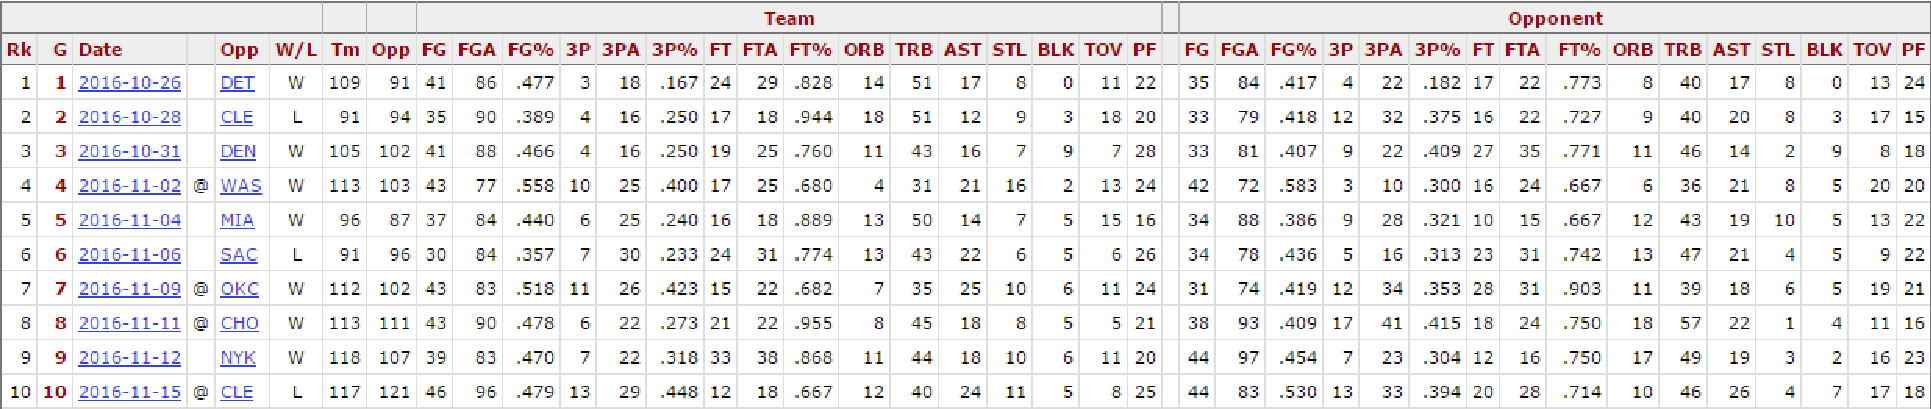
\includegraphics[width=1\textwidth]{{Figures/raptors_gamelog.pdf}}
\captionof{figure}{Game Logs of the Toronto Raptors in the 2016-2017 Regular Season \citep{basketball_reference}}
\label{fig:game_logs}
\end{figure}

\begin{figure}[h]
\centering
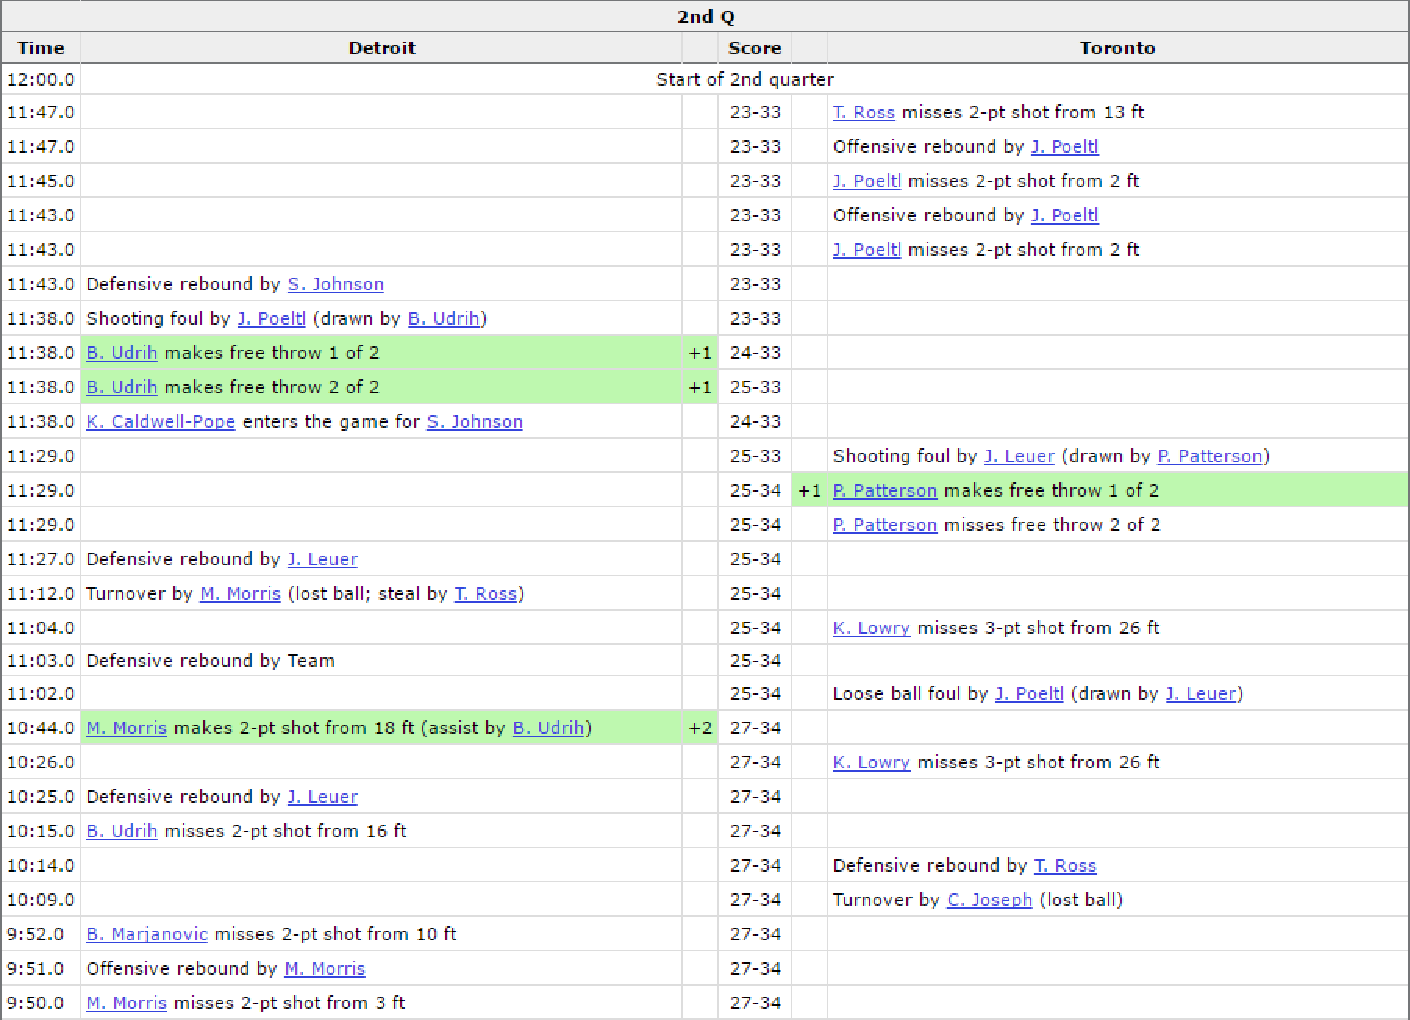
\includegraphics[width=1\textwidth]{{Figures/raptors_pbp.pdf}}
\captionof{figure}{Snippet of the play by play between Toronto and Detroit}
\label{fig:play_by_play}
\end{figure}
	% Appendix Title

\chapter{Dixon Coles}


\section{Dixon and Coles}

\begin{table}[t]
\centering
\caption{Parameter estimates from the 2014, 2015 and 2016 NBA season using the Dixon Coles model implemented for Basketball}
\begin{tabular}{|l|c|c|}
\hline
\textbf{Team}  & \textbf{$\hat{\alpha}$} & \textbf{$\hat{\beta}$} \\ \hline
Atlanta Hawks  & 100.902 & 0.985\\ \hline
Boston Celtics & 99.962 & 1.010\\ \hline
Brooklyn Nets  & 97.400 & 1.013\\ \hline
Charlotte Hornets & 96.978 & 0.976\\ \hline
Chicago Bulls & 97.688 & 0.969\\ \hline
Cleveland Cavaliers & 101.066 & 0.990\\ \hline
Dallas Mavericks & 102.960 & 1.008 \\ \hline
Denver Nuggets & 101.646 & 1.038\\ \hline
Detroit Pistons & 99.256 & 1.012\\ \hline
Golden State Warriors & 108.000 & 0.995\\ \hline
Houston Rockets & 104.750 & 1.017 \\ \hline
Indiana Pacers & 97.358 & 0.957 \\ \hline
Los Angeles Clippers & 104.578 & 0.984\\ \hline
Los Angeles Lakers & 98.553 & 1.052 \\ \hline
Memphis Grizzlies & 95.980 & 0.947\\ \hline
Miami Heat & 97.829 & 0.969\\ \hline
Milwaukee Bucks & 96.464 & 1.006\\ \hline
Minnesota Timberwolves & 101.166 & 1.038\\ \hline
New Orleans Pelicans & 99.337 & 1.007\\ \hline
New York Knicks & 95.207 & 0.996\\ \hline
Oklahoma City Thunder & 105.347 & 1.000\\ \hline
Orlando Magic & 97.111 & 1.015\\ \hline
Philadelphia 76ers & 95.430 & 1.0518\\ \hline
Phoenix Suns & 101.608 & 1.027\\ \hline
Portland Trail Blazers & 103.534 & 1.002\\ \hline
Sacramento Kings & 101.560 & 1.040\\ \hline
San Antonio Spurs & 102.417 & 0.943\\ \hline
Toronto Raptors & 101.480 & 0.984 \\ \hline
Utah Jazz & 94.453 & 0.956\\ \hline
Washington Wizards & 99.983 & 0.999\\ \hline
\multicolumn{2}{|c|}{\textbf{Home Court Advantage}} & 1.025\\ \hline
\end{tabular}
\label{table:dc_141516}
\end{table}

\section{Dixon and Robinson}

\begin{table}[t]
\centering
\caption{Dixon and Robinson model I basketball estimates from the 2014,2015,2016 NBA season}
\begin{tabular}{|l|c|c|}
\hline
\textbf{Team}  & \textbf{$\hat{\alpha}$} & \textbf{$\hat{\beta}$} \\ \hline
Atlanta Hawks  & 101.111 & 0.988\\ \hline
Boston Celtics & 99.962 & 1.010\\ \hline
Brooklyn Nets  & 97.487 & 1.015\\ \hline
Charlotte Hornets & 96.995 & 0.975\\ \hline
Chicago Bulls & 97.321 & 0.969\\ \hline
Cleveland Cavaliers & 101.001 & 0.992\\ \hline
Dallas Mavericks & 102.111 & 1.008 \\ \hline
Denver Nuggets & 101.703 & 1.041\\ \hline
Detroit Pistons & 99.170 & 1.011\\ \hline
Golden State Warriors & 108.163 & 1.001\\ \hline
Houston Rockets & 104.696 & 1.020 \\ \hline
Indiana Pacers & 97.259 & 0.963 \\ \hline
Los Angeles Clippers & 104.787 & 0.992\\ \hline
Los Angeles Lakers & 99.906 & 1.063 \\ \hline
Memphis Grizzlies & 96.038 & 0.962\\ \hline
Miami Heat & 98.005 & 0.962 \\ \hline
Milwaukee Bucks & 96.272 & 1.008\\ \hline
Minnesota Timberwolves & 101.109 & 1.038\\ \hline
New Orleans Pelicans & 99.506 & 1.010\\ \hline
New York Knicks & 95.359 & 0.996\\ \hline
Oklahoma City Thunder & 105.371 & 1.003\\ \hline
Orlando Magic & 96.964 & 1.014\\ \hline
Philadelphia 76ers & 95.559 & 1.058\\ \hline
Phoenix Suns & 101.902 & 1.032\\ \hline
Portland Trail Blazers & 103.242 & 1.004\\ \hline
Sacramento Kings & 101.531  & 1.042\\ \hline
San Antonio Spurs & 102.589 & 0.946\\ \hline
Toronto Raptors & 101.163 & 0.985 \\ \hline
Utah Jazz & 94.245 & 0.963 \\ \hline
Washington Wizards & 99.470  & 0.997\\ \hline
\multicolumn{2}{|c|}{\textbf{Home Court Advantage}} & 1.028\\ \hline
\end{tabular}
\label{table:dr_1_141516}
\end{table} % Appendix Title

%\input{Appendices/AppendixC} % Appendix Title

\addtocontents{toc}{\vspace{2em}}  % Add a gap in the Contents, for aesthetics
\backmatter

%% ----------------------------------------------------------------
\label{Bibliography}
\lhead{\emph{Bibliography}}  % Change the left side page header to "Bibliography"
\bibliographystyle{unsrtnat}  % Use the "unsrtnat" BibTeX style for formatting the Bibliography
\bibliography{Bibliography}  % The references (bibliography) information are stored in the file named "Bibliography.bib"

\end{document}  % The End
%% ----------------------------------------------------------------